%!TEX root = ../Bachelorarbeit.tex
\chapter{Motivation}
\label{chap:Einleitung}
Die HPI School of Design Thinking lehrt die kreative Herangehensweise an Probleme und die Entwicklung einfallsreicher Lösungen. Die Lehre findet dabei in verschiedenen Kursen statt. Studierende können sich die Grundlagen im \gls{Basic-Track} aneignen und ihr Wissen nach erfolgreicher Absolvierung im  \gls{Advanced-Track} vertiefen. Neben den studentischen Kursen bietet die D-School auch Weiterbildungskurse für Unternehmen an.

In der Regel besteht ein Design Thinking-Kurs aus mehreren multidisziplinären Kleingruppen von üblicherweise sechs Teilnehmern, die gemeinsam an einem Projekt arbeiten. Das Projektthema wird dabei entweder von der D-School selbst oder, vor allem bei längeren Projekten, von externen Projektpartnern vorgeschlagen. 

Bei der Arbeit an einem Projekt durchlaufen die Teilnehmenden verschiedene Phasen, die in der Abbildung \ref{fig:dschool-prozess} dargestellt sind: Während zunächst das Verstehen und Beobachten des Problemfeldes im Vordergrund stehen, wird anschließend ein Standpunkt definiert. Es folgt die Phase der Ideenfindung, an die die Erstellung eines Prototypen anknüpft. Dieser Prototyp wird abschließend mit geeigneten Versuchspersonen getestet (vgl. \cite{design-thinking}). Dabei entstehen im Verlauf der Phasen unterschiedliche Dokumente, welche die Lösungsfindung dokumentieren.

\begin{figure}[ht]  
  \centering     
  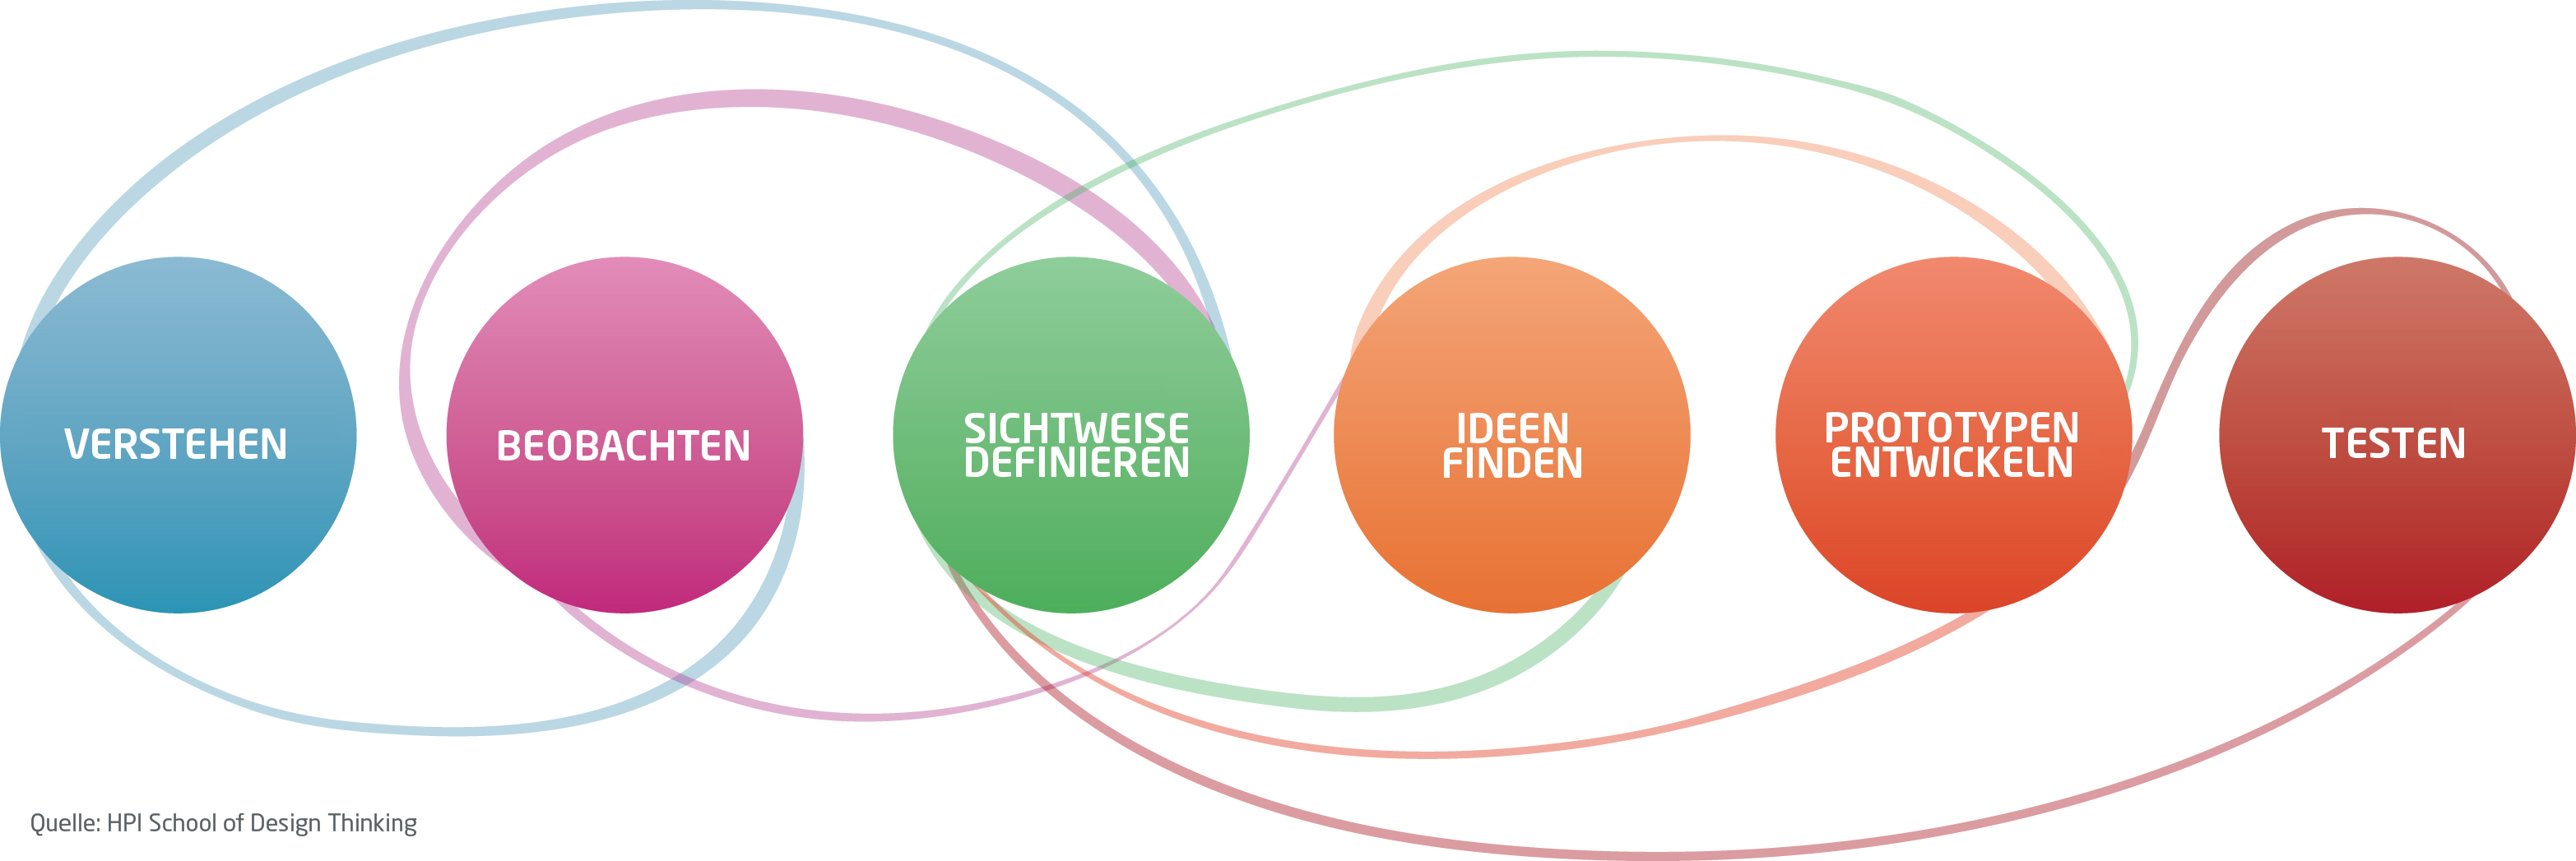
\includegraphics[width=1.0\textwidth]{img/dschool_prozess.jpg}  
   \caption{Phasen des D-School-Prozesses\protect\footnotemark}
  \label{fig:dschool-prozess} 
\end{figure}
\footnotetext{Quelle \cite[p.~114]{design-thinking}}

Im Verlauf des Projektes kommt es durchaus vor, dass ein Team eine Phase mehrmals durchläuft oder in eine vorherige Phase zurückkehrt. Dies erschwert die Organisation der Dokumente, z.B. in einer einfachen hierarchischen Struktur. Weiterhin ist es schwierig, allein aus den Dokumenten deren Entstehungsreihenfolge und Bedeutung zu erfassen. Meist entstehen während eines drei Monate andauernden Projektes verschiedenste Präsentationen, Zusammenfassungen, Prototypen, Bilder von Whiteboards und Interviewdokumentationen. Diese werden in der Regel in der von den Studierenden bevorzugten Art und Weise gespeichert und verwaltet, beispielsweise mit Hilfe von \tete{Dropbox}\footnote{Dropbox, \url{http://www.dropbox.com} (Zugriff 13.06.13)}, \tete{Google Docs}\footnote{Google Docs, \url{http://drive.google.com} (Zugriff 12.06.13)} oder \tete{\gls{Box}}\footnote{Box, \url{http://box.com} (Zugriff 13.06.13)}.

Das Verständnis der Dokumentation ist sowohl für das Projekt selbst, zum Verstehen und Erlernen des Prozesses, als auch als Ideenquelle für zukünftige Projekte wichtig. Ferner sind die erstellten Artefakte nützlich, um neue Projektpartner anzuwerben, welche zukünftige Projekte anbieten. 

\section{Systemanforderungen}
\label{sec:requirements}

Im Verlauf des Projektes wurden in Zusammenarbeit mit den Mitarbeitern und Studierenden der D-School verschiedene Anforderungen an Project-Zoom als Projektverwaltungs- und Dokumentationstool aufgestellt (vgl. \cite{requirements}).  Aus diesen leiten sich die umgesetzte Architektur und die verwendeten Technologien ab. In dieser Arbeit aufgeführt sind nur die für diesen Teil des Projektes wichtigsten und relevanten Anforderungen. Für eine Analyse der Nutzergruppen und deren Bedürfnisse sei auf \cite{requirements}  verwiesen.

\paragraph{Funktionale Anforderungen}
\label{sec:functional}
\begin{labeling}{\textbf{NF1:}}
  \item[F1\label{itm:f1}] Es muss sichergestellt werden, dass kein unautorisierter Nutzer auf Daten Zugriff hat, die geschützt sind.

  Dies ergibt sich aus dem Vorhandensein von Geheimhaltungsverträgen (NDA) für Projekte und dem Wunsch der D-School den Zugriff auf Projekte einzuschränken. 

  \item[F2\label{itm:f2}] Innerhalb der Anwendung sollen die Daten aus \tete{Filemaker}\footnote{Filemaker ist die Datenbank, welche die D-School verwendet um Projekt und Userdaten zu speichern.\\ \url{http://www.filemaker.com} (Zugriff 29.06.13)}, Box, Netzwerkdateisystemen\footnote{Ein Netzwerkdateisystem ist ein Dateisystem, auf welches von Rechnern im selben Netzwerk zugegriffen werden kann, um zum Beispiel Dateien zu lesen.} und \tete{Facebook}\footnote{The Facebook, \url{http://www.facebook.com} (Zugriff 29.06.13)} aggregiert werden.

  Die angegebene Reihenfolge entspricht dabei dem Wunsch der Umsetzung von der D-School.
\\ %FIX TO GET ON A NEW PAGE
  \item[F3\label{itm:f3}] Aggregierte Daten sollen nicht gelöscht werden. 

  Es kann durchaus vorkommen, dass Daten in aggregierten Quellen nach einiger Zeit gelöscht werden müssen. Die Anwendung soll die Daten dann weiterhin vorhalten können. Dass eine Ressource in der originalen Quelle nicht mehr vorhanden ist, kann zum Beispiel durch eine Markierung in einer Datenbank erfolgen.

  \item[F4\label{itm:f4}] Die Anbindung von neuen Datenquellen muss möglich sein. Das Core-Backend soll dabei unverändert bleiben.

  Über die Zeit wandeln sich die von den Studierenden verwendeten Werkzeuge zur Dokumentation. Dies muss bei der Anwendungskonzeption berücksichtigt werden.

  \item[F5\label{itm:f5}] Es dürfen keine aggregierten Daten in deren Quellen verändert werden.

  Die Anwendung soll auf externe Daten nur lesend zugreifen. Dies dient dem Schutz der Datenquellen.

  \item[F6\label{itm:f6}] Die Studierenden sollen in der Lage sein, die Anwendung außerhalb der D-School verwenden zu können. 

  Dies ist wichtig, da die Studierenden meist nur zwei Tage in der Woche in der D-School verbringen. Zum Teil treffen sich die Projektteilnehmer außerhalb der D-School mit Interview- und Projektpartnern, welche am Stand des Projektes interessiert sind. 
\end{labeling}

\paragraph{Nichtfunktionale Anforderungen}
\label{sec:nonfunctional}

\begin{labeling}{\textbf{NF1:}}
  \item[NF1\label{itm:nf1}] Es sollen 100 Nutzer gleichzeitig in der Lage sein, das Backend zu nutzen.

  Dies Angabe entsteht aus der Abschätzung für die maximale Anzahl aller Teilnehmer und Lehrenden von etwa 100 Nutzern. Da keine anderen Nutzer Zugriff auf das System haben sollen, entspricht dies einer oberen Schranke für die Anzahl der aktiven Nutzer. 

  \item[NF2\label{itm:nf2}]  Der Server muss die Updates aus den Datenquellen innerhalb von einer Minute verarbeiten.

  Umso schneller die Updates vom System verarbeitet werden, desto eher können die Nutzer mit den Daten in der Anwendung arbeiten. Die Grenze von einer Minute wurde gewählt, da dies einerseits eine realistische Zeitspanne für notwendige Berechnungen ist und andererseits den Studierenden das reibungslose Arbeiten mit dem System ermöglicht.
\end{labeling}


\section{Idee von Project-Zoom}
 
Im Entwicklungsprozess einer Lösung zur Verbesserung der Dokumentation in der D-School wurde auf den D-School-Prozess zurückgegriffen. Diese Vorgehensweise ermöglichte einen sehr guten Einblick in die Arbeitsweise der Teilnehmer in den Projekten der D-School. 

\begin{figure}[ht]  
  \centering     
  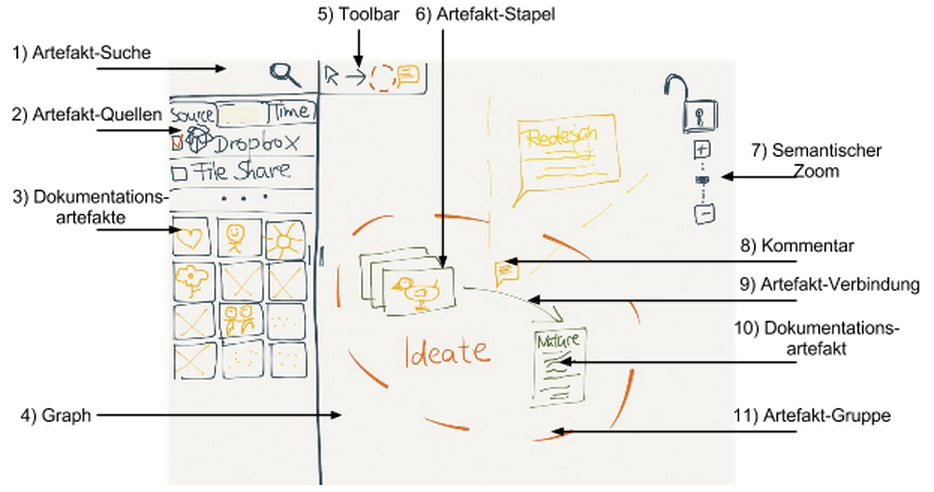
\includegraphics[width=1.0\textwidth]{img/projectzoom_prototype.png}  
   \caption{Prototyp einer Übersicht über den Dokumentationsprozess eines Projektes}
  \label{fig:projectzoom_prototype} 
\end{figure}

In mehreren Iterationen wurde Project-Zoom entwickelt und verfeinert. Einer der ersten Entwürfe der Nutzoberfläche ist in Abbildung \ref{fig:projectzoom_prototype} zu sehen. Das Konzept von Project-Zoom ist die Verbindung einer Projektübersicht mit einem Projekteinblick. Der Nutzer soll die Möglichkeit haben, einen Überblick über alle Projekte, und bei Bedarf einen tieferen Einblick in ein konkretes Projekt, zubekommen.

Project-Zoom soll der Verbesserung der Dokumentation dienen. Dazu sollen die von den Studierenden erzeugten Artefakte durch manuelles Anordnen in eine Form gebracht werden, welche den Prozess der Gruppe visualisiert. Die Mitarbeiter der D-School können die entstandenen Graphen anschließend nutzen, um die Projektverläufe zu analysieren und gegebenenfalls Abläufe innerhalb einer Design Thinking-Phase anzupassen (vgl. Interview mit Claudia Nikolai im Anhang \ref{sec:interview_nikolai}).

Für eine reibungslose Integration des Systems ist vor allem die Anbindung an bereits existierende IT-Systeme  und die von den Studierenden für das Projekt verwendete Software wichtig (vgl. Anforderung \ref{itm:f2}). Änderungen an diesen externen Diensten und der Auswahl der anzubindenden Datenspeicher ist über die Zeit sehr wahrscheinlich. Deshalb muss das System modular aufgebaut sein, um nachträglich neue Dienste anbinden zu können, ohne den Backend-Core zu verändern.

\section{Abgrenzung}
Die Arbeit beschreibt und bezieht sich auf das Bachelorprojekt „From Creative Ideas to Well-Founded Engineering“ und das umgesetzte Softwaresystem Project-Zoom. Insgesamt haben sechs Studierende an dem Projekt gearbeitet, die in ihren Bachelorarbeiten Project-Zoom aus verschiedenen Blickwinkeln und mit verschiedenen Schwerpunkten beschreiben.

Tom Herolds Arbeit \cite{bp-tomh} beinhaltet die Interaktion mit kontextsensitiven Graphen. Dabei geht es darum, den Umgang der Studierenden mit der Nutzeroberfläche so intuitiv wie möglich zu gestalten und den Nutzer bei der Erfassung dokumentationsrelevanter Eigenschaften zu unterstützen.

Die Ausführungen von Anita Diekhoff \cite{bp-anita}  beschäftigen sich mit der Übersicht über Projekte und gehen näher auf Layoutfunktionalitäten in interaktiven Graphen ein.

Norman Rzepkas Bachelorarbeit \cite{bp-norman} thematisiert die webbasierte, eventgesteuerte, clientseitige Architektur von Project-Zoom. Dabei wird näher darauf eingegangen, wie die Daten von der Datenbank über das Backend asynchron an den Client ausgeliefert und angezeigt werden.

Die Arbeit von Dominic Bräunlein \cite{bp-dome} erläutert das Generieren und Bereitstellen von semantischen \gls{Thumbnails}, um dem Nutzer das Erkennen der Dokumente seines Projektes zu erleichtern und somit selbst bei wenig verfügbarem Platz so viele Informationen eines Dokumentes anzeigen zu können wie möglich. 

Thomas Werkmeisters Arbeit \cite{bp-tewe} befasst sich mit der Anbindung externer Systeme zur Integration von Daten. Diese aggregierte Datenbasis ist die Grundlage für die Wissensbasis und die einzelnen Projekte.

\begin{figure}[ht]  
  \centering     
  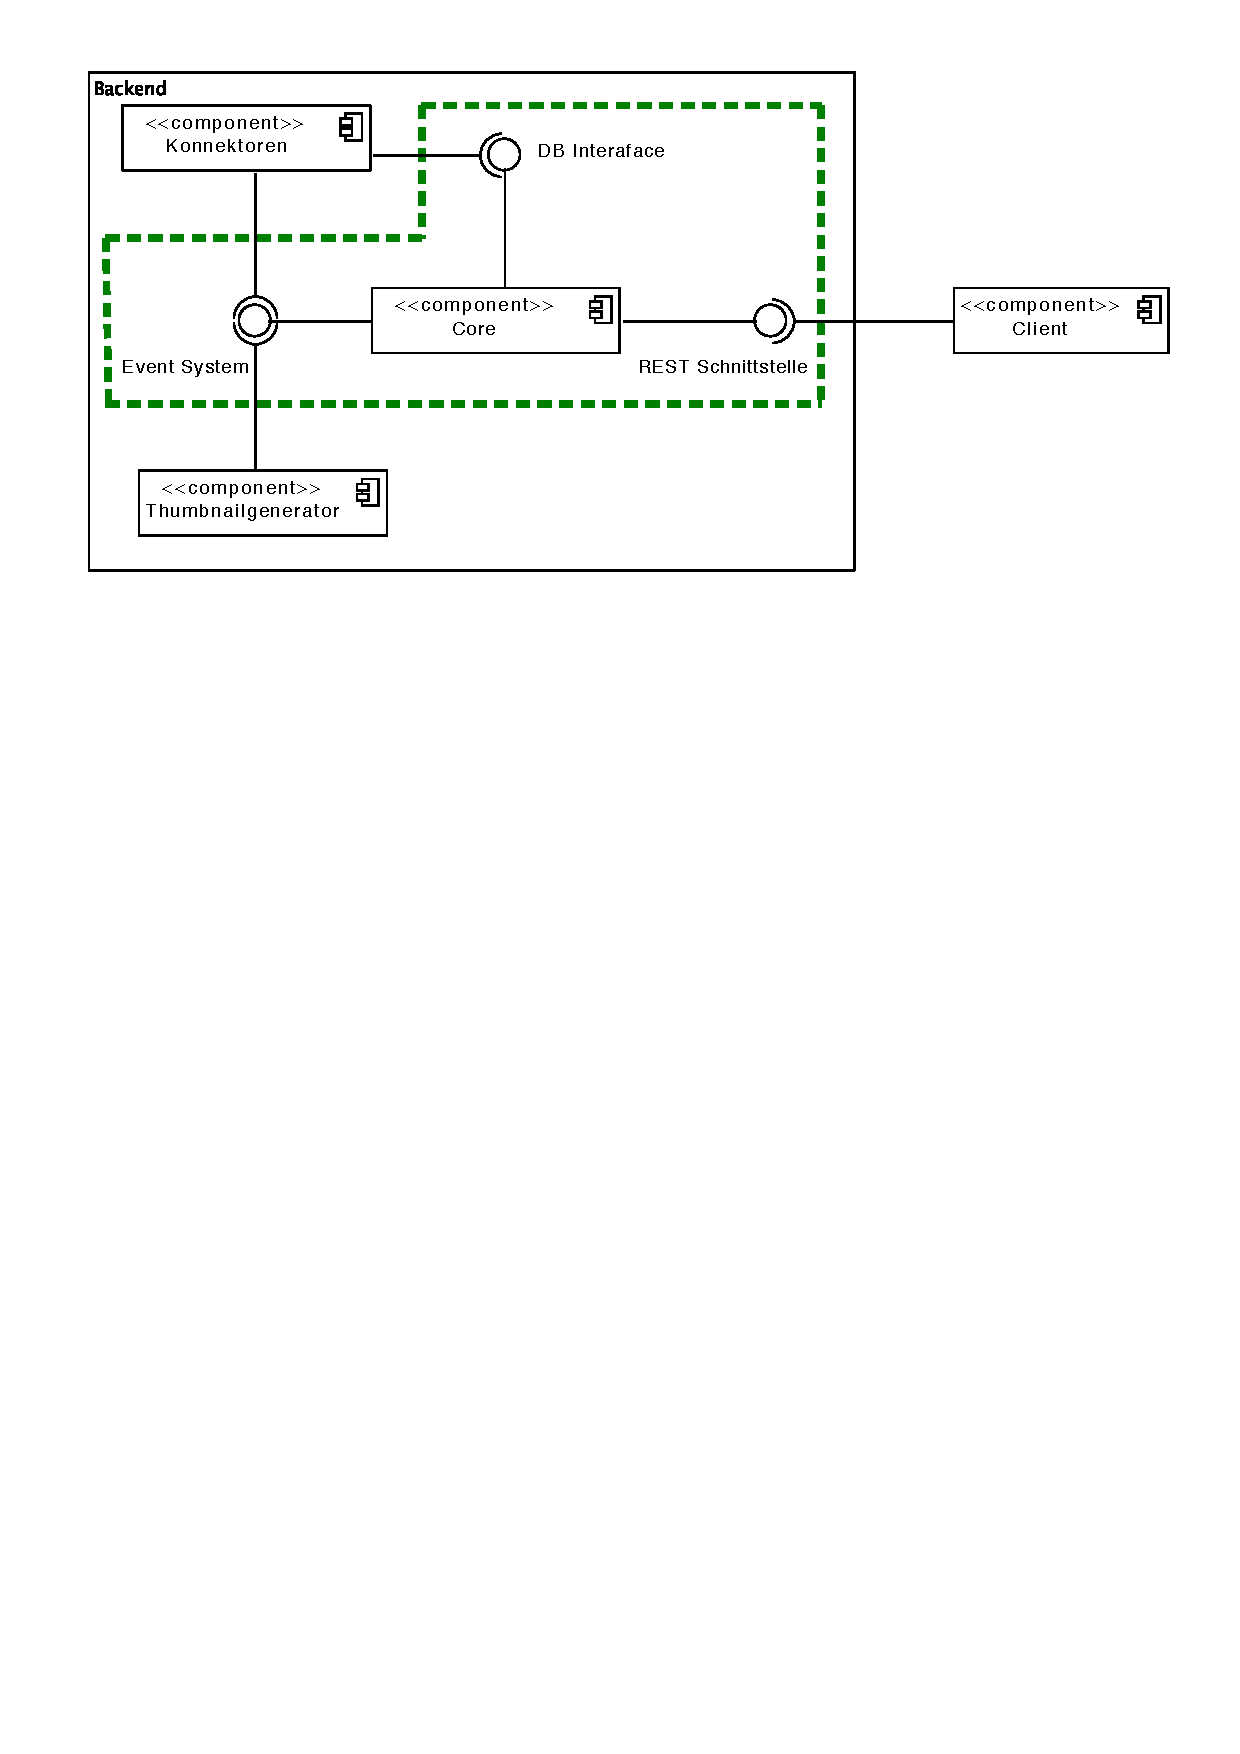
\includegraphics[width=1.0\textwidth]{img/architecture_overview.pdf}  
   \caption{Überblick über die verschiedenen Pakete und ihre Schnittstellen; in dem gestrichelten Rahmen der für diese Arbeit relevante Teil der Architektur}
  \label{fig:architecture-overview} 
\end{figure}

Die Abbildung \ref{fig:architecture-overview} zeigt einen groben Überblick über die Architektur des Systems. Der für diese Arbeit relevante Teil ist dabei durch einen gestrichelten Rahmen gekennzeichnet. Die Komponenten, die in den Arbeiten \cite{bp-tewe} (Konnektoren) und \cite{bp-dome} (Thumbnailgenerator) beschrieben sind, sind mit dem hier erläuterten Systemteil mittels eines Eventsystems verbunden. Das Client-Frontend ist über eine REST-Anbindung\footnote{vgl. Konzept des Representational State Transfer in \cite{rest}} an das Server-Backend angeschlossen. Mit der clientseitigen Implementierung der REST-Schnittstelle beschäftigt sich \cite{bp-norman}.

In dieser Arbeit wird zunächst ein Überblick über das Gesamtsystem gegeben. Dazu werden die Anforderungen der D-School an das Backend analysiert, welche als Grundlage für die Wahl der verwendeten Technologien dienen. Anschließend wird die Architektur des Backends näher erläutert. Hier liegt der Hauptfokus zunächst auf einer neuen Art und Weise, eine Datenbank an eine Webapplikation anzubinden. Im Anschluss werden einige Feinheiten und ausgewählte Stellen der Datenmodellierung von Project-Zoom beleuchtet. Den Abschluss bildet die architekturelle Grundlage zur Anbindung externer Systeme für die Erweiterung von Project-Zoom.